\chapter{Conceptual Overview of Reinforcement Learning Techniques applied to CRS}
\chaptermark{Reinforcement Learning Techniques applied to CRS}
\label{ch:rl_crs} 

\section{CRS Interfaces}
Broadly speaking, all CRS can be divided into chatbots (systems with natural language interface) and other interactive applications, typically webpages, which use various display and control elements, such as buttons, hyperlinks, images, descriptions, and carousels to interact with the user \citep{jannach2021survey}.

For the most part, reinforcement learning research in CRS focuses on non-chatbot applications that optimise such elements as web page user flow \citep{mahmood2009improving, mahmood2009learning}, order of items in recommendation lists \citep{viappiani2009regret}, sequential item recommendations, like the ones that can be found on music or video streaming sites \citep{zhao2013interactive}, or interactive critique elicitation dialogues, where users are asked to rate (like or dislike) items or indicate their preference among sets of two or multiple options \citep{christakopoulou2016towards}. Some such systems are trained and tested in reinforcement learning gyms with no specific interface in mind \citep{sun2018conversational, lei2020estimation, li2021seamlessly}. These types of systems are typically focused purely on recommendation quality. 

Natural language based systems are substantially less common \citep{greco2017converse, sun2018conversational, tsumita2019dialogue, kang2019recommendation, wang2022improving, zhou2022c2}. These systems typically aim to achieve a more natural, human-like interaction and include side goals such as chit-chat. These systems are typically more complex and require additional modules, such as encoder and decoder, ranging in complexity from seq2seq \citep{greco2017converse} to state-of-the-art neural language models like BART \citep{wang2022improving}. Authors of such systems place the focus on quality of utterances and use NLP specific evaluations such as Bilingual Evaluation Understudy (BLEU) \citep{greco2017converse} and qualitative evaluations such as real user feedback \citep{kang2019recommendation}. For this reason, quality of recommendations is seen as a secondary goal and is less important than in non-chatbot systems.

\section{Typical Architecture of a Reinforcement Learning Driven CRS}

CRS architectures vary widely depending on application and methodology, however, there are a number of components that are typical for most CRS \citep{jannach2021surve, pramod2022conversational}. Figure~\ref{fig:crs_architecture} illustrates these components and their interactions.

\begin{figure}[ht]
    \centering
    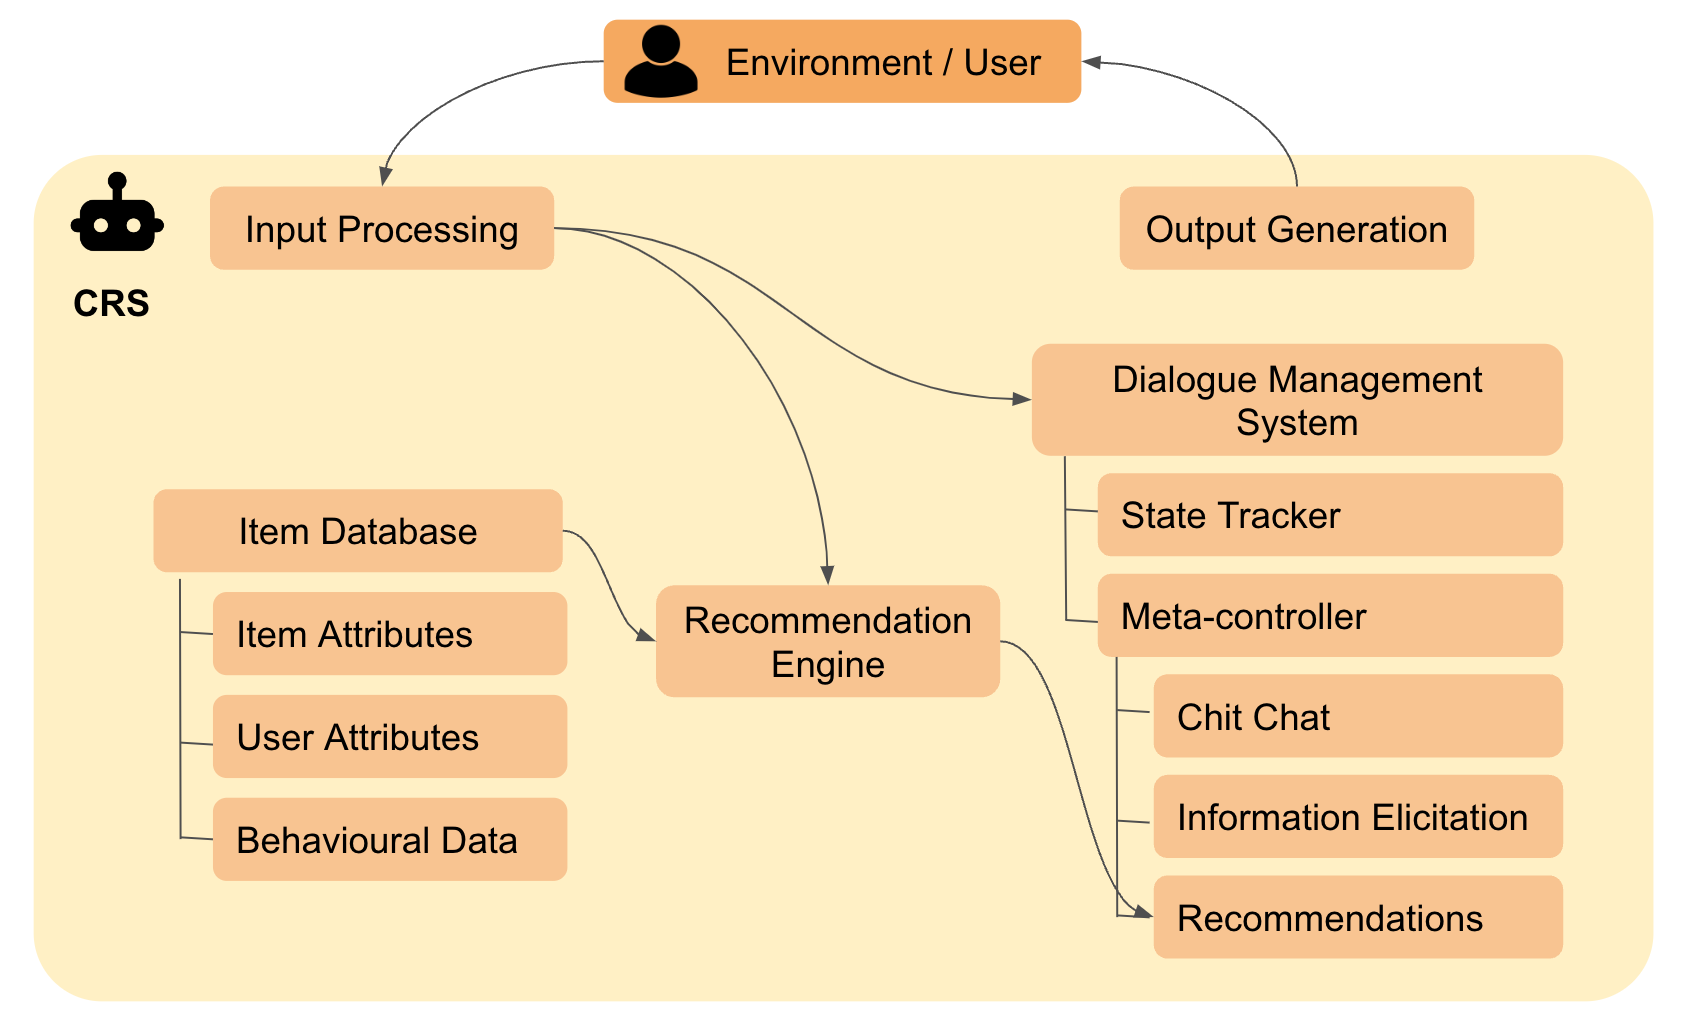
\includegraphics[scale=0.22]{figures/crs_architecture.png}
    \caption{Typical architecture of a CRS}
    \label{fig:crs_architecture}
\end{figure}

\begin{itemize}
    \item Environment. All CRS interact with a real or a simulated user, which is operationalised as an environment in reinforcement learning applications \citep{mahmood2009learning, tsumita2019dialogue}.

    \item Input Processing Module. Some CRS, particularly the ones that are driven by an interactive interface (hyperlinks, buttons, carousels) do not require an explicit input processing module, as they can directly ingest user action events \citep{mahmood2009learning, mangili2020bayesian}. In contrast, CRS that operate as chatbots require a natural language understanding (NLU) module in order to process user utterances and extract information such as attribute-value pairs, user intentions or encode full sentences \citep{sun2018conversational, kang2019recommendation, tsumita2019dialogue, wang2022improving, zhou2022c2}. Typically such modules require some degree of supervised training or pretraining on real or simulated datasets in order to cope with the diversity of natural language. Some such systems are further fine-tuned with reinforcement learning on either rule-based gym environments \citep{sun2018conversational} or through bot-play \citep{kang2019recommendation}.

    \item Output Generation Module. Similarly to the input module, an output module may or may not involve natural language processing depending on the interface of the system. While some chatbot applications use natural language generation to produce natural and varied agent utterances \citep{kang2019recommendation, sun2018conversational, wang2022improving, zhou2022c2}, others produce templated responses or simply output preference elicitation items or rank-ordered recommendation lists as interactive interface elements \citep{sun2018conversational, lei2020estimation}.

    \item Item Database. Nearly all CRS are pre-trained based on collaborative user-item datasets, which are often enriched with item attribute metadata \citep{mahmood2008adaptive}.

    \item Recommendation Engine. Recommendation module is ubiquitous in CRS and is usually trained based on established recommender techniques, such as Matrix Factorisation \citep{zhao2013interactive, christakopoulou2016towards} or Factorisation Machines \citep{sun2018conversational, lei2020estimation, li2021seamlessly} and are sometimes fine-tuned using reinforcement learning \citep{tsumita2019dialogue}.

    \item Dialogue Management System. Last but not least, all CRS include some version of a dialogue management system, which keeps track of the dialogue state and determines the policy under which the CRS operates. The Dialogue Management System is the primary component to be trained and optimised with reinforcement learning techniques \citep{tsumita2019dialogue}. The Policy module is sometimes subdivided into a meta-controller, which outputs a probability distribution over high-level goals (e.g., chit-chat vs recommendation), and controllers dedicated to individual sub-goals, which select specific actions \citep{greco2017converse}. A substantial body of research focuses on designing dialogue management systems capable of finding an optimal balance between eliciting preferences and offering recommendation in order to learn and exploit user requirements efficiently \citep{sun2018conversational, li2021seamlessly}.
\end{itemize}

\section{Preference Elicitation in Conversational Recommender Systems}
\subsection{Preference Elicitation Strategies}

\textit{CRS} employ different communication strategies. While some systems use a predetermined list of questions, more sophisticated approaches direct a dialogue by actively probing users for the information that is most valuable in a given context \citep{sun2018conversational, christakopoulou2016towards}. The latter approach raises the problem of finding the optimal ‘probing’, or \textit{preference elicitation}, strategy, which allows to gather information that is most useful for generating relevant recommendations in the least number of conversational turns. 

Some \textit{CRS} do not distinguish between preference elicitation (acquiring information from a user) and recommendation tasks. For instance, sequential recommendation systems simultaneously offer items for users to consume and collect user critiques on these items (typically, in the form of interaction with like/dislike buttons) \citep{zhao2013interactive}. It is important for such systems to carefully balance exploration and exploitation in order to achieve sufficient user engagement both in the short term, by making each item recommendation as relevant as possible, and in the long term, by discovering full spectrum of user preferences. This requirement makes sequential CRS a good use case for application of reinforcement learning techniques.

Most \textit{CRS}, however, operationalise preference elicitation and recommendation as two separate tasks. These systems can be broadly divided into critique based systems and attribute driven systems \citep{jannach2021survey, pramod2022conversational}. 

Critique based systems present users with item options and utilise their feedback to update user preference vectors \citep{viappiani2009regret, christakopoulou2016towards, vendrov2020gradient}. Typically, critique based \textit{CRS} rely on collaborative filtering recommendation methods to produce recommendations. Critique systems lend themselves well to bandit algorithms that operationalise items as arms and users as contexts.

Attribute driven systems either present users with item attributes (also called facets) and collect user feedback or mine for attribute-value pairs in user utterances \citep{mahmood2009improving, sun2018conversational, tsumita2019dialogue, kang2019recommendation}. Typically, attribute values are used to narrow down the set of possible recommendations, which are then ranked using collaborative filtering techniques. Attribute driven CRS can be fairly simple in their design. For example, in their experiments Mahmood et al. use a web-based interface that allows users to filter items based on their attributes and then use reinforcement learning techniques to decide whether to recommend additional attributes to prompt users to narrow down the result set even further, in situations where too many matches are returned \citep{mahmood2009improving, mahmood2008adaptive, mahmood2007learning, mahmood2008adapting}. On the other end of the spectrum, some CRS enable users to freely and proactively specify their requirements in natural language, which requires an NLU module in order to extract attribute-value pairs from user utterances \citep{kang2019recommendation, sun2018conversational, tsumita2019dialogue}. These systems typically rely more heavily on supervised learning based on natural datasets. Other systems may focus on discovering the most entropy minimising attributes and present them to users via interactive dialogue screens in web applications or closed yes/no type questions in chatbot applications.

State-of-the-art \textit{CRS} applications are capable of seamlessly combining item attributes and critique methods in order to achieve optimal performance. \textit{Factorisation Machines} tend to be a preferred recommender algorithm to support these types of \textit{CRS}, as they allow to simultaneously obtain embeddings for items, item attributes and users \citep{li2021seamlessly}. A recent study of natural human conversations about movie preferences revealed that humans tend to share examples of movies that they liked or disliked, as well as use generalisations and descriptions of movie attributes \citep{radlinski2019coached}. Combining attributes with items is a promising direction in \textit{CRS} research, as it closely mimics a habit of mixing and matching both types of questions in natural human conversations. 

\subsubsetion(Switching Between Preference Elicitation and Recommendation)
The overarching goal of most CRS is to maximise the probability of a successful dialogue, where success is defined as acceptance of a recommendation \citep{vendrov2020gradient, lei2020estimation, li2021seamlessly} or, in commercial systems, conversion, which is defined as accomplishing the desired goal, such as making a purchase \citep{mahmood2008adaptive, mahmood2009improving, mahmood2009learning}. As users always can quit the dialogue early, interactions that are too lengthy and cognitively taxing will have a lower success rate. On the other hand, inability to elicit sufficient volume of information from users will result in less appropriate recommendations, which, in turn, will also result in low success rate.  

To address the trade-off between information gain and avoidance of user fatigue, some algorithms have employed a rule based approach for determining the point when to switch from questioning to recommendation presentation \citep{christakopoulou2016towards}, while many others have proposed various reinforcement learning techniques \citep{mahmood2009learning, greco2017converse, sun2018conversational, tsumita2019dialogue, vendrov2020gradient, lei2020estimation,  li2021seamlessly}. To achieve the optimal balance, typical reinforcement learning setups penalise CRS for each conversational turn, which results in shorter dialogues \citep{tsumita2019dialogue, lei2020estimation}.

For example, \citep{mahmood2009improving, mahmood2009learning} have shown in a real user study that applying an adaptive system trained with RL shortened the overall interaction time by 50\% compared to a system based on handcrafted rules, while resulting in better conversion. They demonstrate that the adaptive system learns to proactively offer query tightening criteria to users when it helps to reduce cognitive load and skips this step when it is redundant. Similarly, \citep{sun2018conversational} show that an adaptive system capable of flexibly determining when to stop the preference elicitation stage of the dialogue achieves substantially better performance than a system with any fixed number of conversational turns. They argue that a reinforcement learning algorithm is able to detect at which point additional questioning becomes less beneficial in terms of information gain or when risks of user quitting start to outweigh the benefits of collecting additional data.

Further to that, some CRS stop the dialogue at the first recommendation stage whether it has been successful or not \citep{sun2018conversational}. Others are set up as multi-round dialogues, where the system embarks on a new round of information elicitation followed by recommendation until the user either accepts the recommendations or chooses to quit the interaction \citep{lei2020estimation, li2021seamlessly}. This approach is more reflective of real-world requirements, as it places the user in control of the dialogue flow.

\section{Types of Reinforcement Learning Algorithms Used in CRS}
\subsection{Value Function Optimisation Methods}
Early works in the field of reinforcement learning driven CRS feature algorithms that rely on estimation and optimisation of value function Q \citep{henderson2008hybrid, mahmood2007learning, mahmood2008adaptive, mahmood2009improving, mahmood2009learning}. Examples include a SARSA-driven system for optimising travel booking dialogues \citep{henderson2008hybrid} and another MDP-based model proposed by \cite{mahmood2007learning} and later applied in a real-world system \citep{mahmood2008adaptive, mahmood2009improving, mahmood2009learning}.

Value function methods are designed to learn a Markov Decision Process (MDP) policy. MDP is a framework widely used in the field of reinforcement learning. The key elements of MDP are states, actions and rewards. It models decision making in situations where outcomes are partially determined by the agent’s actions and relies on an assumption that each new state in the process depends only on the preceding state. One of the more well-known algorithms in this family is SARSA, used in \cite{henderson2008hybrid}. SARSA evaluates Q-value based on the current state st, agent’s action at, reward r, as well as the next state that the agent transitions to st+1 and the action that the agent will take in the next state at+1. Actions that maximise the Q-value are then selected by the agent as optimal.

\subsection{Policy Gradient Optimisation Methods}
Policy gradient algorithms are commonly used in modern reinforcement learning applications. They forego the calculation of Q-value and instead update the probability distribution of actions in a way that maximises the expected reward. Policy gradient functions are often used to train neural models through gradient ascent. 

REINFORCE is a ubiquitous technique in this family of algorithms and is used widely in the latest CRS works, particularly the ones that focus on building natural language based systems. For example, \cite{greco2017converse} use REINFORCE to optimise utterances produced by the CRS agent, \cite{sun2018conversational} use it to train their Dialogue Management module, which selects an action given the dialogue state after pre-training with entropy method, and \cite{kang2019recommendation} use it to fine-tune their CRS through bot-play after it has been trained with supervised learning.

\subsection{Multi-Armed Bandit Algorithms}
A substantial proportion of works in the field of CRS focus on multi-armed bandit driven algorithms \citep{zhao2013interactive, christakopoulou2016towards,  li2021seamlessly}. Bandit algorithms define actions as ‘arms’ and are optimised to find the arms that maximise the expected gain given the context (e.g., user or item attributes, consumption history), where outcomes of ‘pulling’ each ‘arm’ are only partially known and are gradually revealed as the agent interacts with the environment. Therefore, bandit algorithms offer a range of techniques that address the exploration-exploitation trade-off problem and provide efficient strategies for discovering the best actions from the pool of many possible choices. Recommendation problems can be mapped well onto bandit algorithms, as items available for recommendation can be easily operationalised as arms. 

For example, \cite{zhao2013interactive} have used several bandit algorithms in conjunction with Matrix Factorisation in order to learn user feature vectors as users rate new items. \cite{li2021seamlessly} have taken a step further and developed an algorithm that leverages Factorisation Machine to project items as well as their attributes in the same space, which allowed them to use the bandit approach for selecting the most effective questions for preference elicitation, selecting the items to recommend, as well as seamlessly switching between the two action types. They show that when the user rates an item negatively, it lowers the score for the item, as well as all other items and their attributes that share similar embeddings. Furthermore, as soon as the system receives user feedback on an item or an attribute, the algorithm discourages further exploration of related arms as probability distribution tightens.

Upper Confidence Bound (UCB) and Thompson sampling are among the most prominent techniques in the multi-armed bandit space. UCB estimates confidence bounds for each arm and selects arms with the highest upper bound values. Where confidence is high, this results in ‘pulling’ high-reward arms, whereas where confidence is low this allows to collect feedback from the environment and shrink the confidence interval. As a result, after a sufficient number of exploration rounds, the algorithm converges on the most rewarding actions. Thompson sampling algorithm balances exploration and exploitation by sampling from a posterior distribution of the reward estimation. Several CRS works have compared UCB and Thompson sampling alongside several other bandit algorithms and found that in some cases UCB \citep{zhao2013interactive} and in others Thompson sampling \citep{li2021seamlessly} outperformed other baselines.

\section{Training of Reinforcement Learning Driven CRS}
\subsection{Reward Definitions}
As reinforcement learning is considered semi-supervised, there is no ground truth optimal behaviour as such for the model to learn. Therefore, it becomes important to design rewards in a way that ensures that the CRS learns efficient dialogue strategies. Some authors have compared multiple reward models \citep{mahmood2007learning, sun2018conversational} and demonstrated that they can influence the strategies that the model favours. For example, \cite{mahmood2007learning} have found that under the assumption that the length of interaction is not related to decrease in dialogue success probability, and so is not penalised, the system learns to not recommend query tightening.

The most common approach for CRS is to assign a large positive reward at the end of the dialogue upon successful dialogue completion (i.e. when the user accepts the recommendation or converts), as well as assign small negative rewards at each conversational turn based on the assumption that longer conversations are less efficient, more cognitively taxing and more likely to result in the user quitting the session \citep{henderson2008hybrid, mahmood2007learning, sun2018conversational, tsumita2019dialogue, lei2020estimation}. Some authors add additional penalties for incoherent or illogical utterances \citep{tsumita2019dialogue} and quitting the dialogue \citep{lei2020estimation} and additional rewards for accepting a suggested item attribute \citep{lei2020estimation}.

Some authors, however, chose different approaches. For instance, \cite{zhao2013interactive} operationalised the reward in their bandit-driven sequential CRS as item rating and \cite{greco2017converse} used a combination of F1 and BLEU score, which allowed to train the system to generate more coherent utterances. Generally, rewards should reflect the specific goals and design of the whole system.

\subsection{Datasets and Algorithm Validation}
Real-world dialogue datasets are still rare in the domain of CRS. Majority of works are trained on collaborative datasets, where the system is interactive interface driven, and simulated user-system dialogues, where natural language approach is used. For example, many researchers use established datasets in the domain of movie recommendations (MovieLens, EachMovie, Netflix) \citep{zhao2013interactive, greco2017converse, vendrov2020gradient}, as well as restaurants (Yelp) \citep{sun2018conversational,  lei2020estimation}, music (LastFM) \citep{li2021seamlessly} and books (Goodreads) \citep{vendrov2020gradient}.

CRS with chatbot interface mainly rely on dialogues synthesised on the basis of the datasets mentioned above \citep{greco2017converse, sun2018conversational}. While some authors simulate the dialogues using a small number of simple templates \citep{greco2017converse}, others endeavor to approximate realistic human language. For example, \cite{sun2018conversational} have commissioned Amazon Mechanical Turk (AMT) workers to generate natural wording examples based on predefined dialogue schemas and recycled them in order to synthesise 876,000 artificial dialogues.

Real user tests are rare and confined to laboratory settings. For example \citep{mahmood2009improving, mahmood2009learning} have implemented their algorithm in a commercial system and tested it on just under 500 users, however, there were some design flaws in the study. Firstly, all users have completed a task on a rule-driven system first and then on the adaptive system, which could have led to the transfer-of-skills bias as well as the survivor bias, since not all users were retained in the stage two of the task, though all were considered in the analysis. Secondly, the users were performing an artificial task of finding a product and adding it to their basket, without having to actually buy it, so external validity of the study is limited.

Another attempt was made by \cite{sun2018conversational} who employed AMT workers to test the algorithm. However, in order to leverage the historical clickstream data of real users, AMT workers were asked to familiarise themselves with the consumption history of a random user drawn from the dataset and guess the recommendation they would have been likely to accept. Similar approach was used by \citep{kang2019recommendation}, who offered a small financial incentive to AMT workers for correctly guessing predefined target items. While this is a step towards validating the algorithms in the real-world scenario, it remains challenging to recreate settings where system effectiveness at improving real user conversion would be evaluated.

\subsection{Pre-training Strategies}
Several authors note that it is difficult to learn optimal system behaviour using reinforcement learning alone \citep{henderson2008hybrid, sun2018conversational}, particularly if the system is natural language based \citep{greco2017converse}. For example, \cite{henderson2008hybrid} observe that a system trained using reinforcement learning only produces unreliable results as suboptimal agent behaviour, such as repetition of the same question even after the information has already been obtained. In contrast, pre-training using supervised learning methods allows to initialise the system with a policy learned on an existing corpus and further improve on it. Similarly, \cite{sun2018conversational} use the entropy method for ranking preference elicitation questions in order to pre-train their model, as random initialisation produces unreliable results. 

In addition to that, some authors leverage large collaborative datasets available to the academic community in order to pre-train recommendation systems offline before using the obtained embeddings in CRS \citep{lei2020estimation,  li2021seamlessly}. For example, \citep{li2021seamlessly} train an offline Factorisation Machine model in order to embed users, items and their attributes in the same space and then use the resulting representations to train a Thompson sampling algorithm.

Pre-training with supervised learning is ubiquitous in natural language driven system, as it is not feasible to learn to generate natural language with reinforcement learning alone. It is typical for such systems to employ various versions of neural encoder-decoder architectures and train them using cross-entropy loss on existing corpora of data (either synthetic or human generated) and then fine-tune the system by replacing cross-entropy loss with REINFORCE \citep{greco2017converse, kang2019recommendation} function.

More recent studies increasing rely on pretrained Large Language Models (LLMs) and their embedded knowledge which extends to various recommendation domains. LLMs are transformer based language models pre-trained on diverse and extensive datasets, which allows them to have a broad understanding of language patterns, grammar, and semantics without or with only minimal fine-tuning. Recent papers utilise the ability of LLMs to reason to replace more traditional recommendation system approaches. For example, \cite{wang2022improving} utilise pre-trained BART model to initialise their CRS, which allows them to discard domain-specific external knowledge sources and rely on entity level and contextual level representations discovered directly from the conversation and contextualised using the pre-existing knowledge encoded LLM.

In recent months several research groups demonstrated state-of-the-art LLMs such as ChatGPT \citep{gao2023chat}, LaMDA \citep{friedman2023leveraging} and LLaMa \citep{bao2023tallrec} are capable to reason about user preferences with minimal or no fine-tuning. \cite{bao2023tallrec} propose a lightweight fine-tuning framework called TALLRec based on  LLaMA model in order to train the LLM to rerank item candidates retrieved by a recommendation module. While they do not focus on semantic and stylistic characteristics of the produced text, they demonstrate LLM ability to achieve quality of ranking comparable with traditional baselines.

Other researchers opt to forego the fine-tuning process altogether and instead adopt a prompt-based injection approach to manipulate the output generated by LLMs and influence the model's behaviour. For example, \citep{gao2023chat} propose a framework called Chat-REC and demonstrate that prompt engineering alone is sufficient to construct a CRS based on the ChatGPT model. They convert user profiles and consumption history into prompts, supplement this information with a shortlist of items produced by a retrieval module and instruct the LLM to do post-recommendation ranking of items. 

Another example from Google research is the RecLLM framework built on the basis of the LaMDA model \citep{friedman2023leveraging} for recommendation of YouTube videos.  The authors apply a chain-of-reasoning approach in order to instruct the LLM to complete multiple functions in a sequence, including dialogue management and recommendation re-ranking. The LLM utilises a combination of the user query and the contextual information from the dialogue to make a decision regarding the appropriate approach for addressing the user's query. For example, when a user specifies desired attributes of a movie clip they want to watch, LLM generates a request to recommendation engine, receives the shortlist of recommended videos and reranks them based on its understanding of user profile and conversation context. LLM is also used to emulate the user.

In general, LLMs are known to be able to process semantically complex texts and reason based on them. \cite{radlinski2019coached} have criticised existing CRS for reliance on the available metadata (genres, categories), while, in the real-world unconstrained scenarios users often use less well defined properties such as story, plot, characters, acting and attributes like violence. LLM based approach makes it possible to maintain such conversation with minimal or no fine-tuning, while being able to support user guided non-linear conversational flows that include preference elicitation, recommendation and providing information to users, while also adding transparency and explainability \citep{gao2023chat, bao2023tallrec}.

\subsection{Environments for Training Reinforcement Learning Algorithms}
In contrast with supervised learning models, reinforcement learning requires feedback from the environment in order to update the parameters, which poses a practical challenge for training CRS. Even those authors that implement their algorithms in commercial systems cannot afford to do the initial training on real users, as an untrained system can demonstrate suboptimal performance, which is commercially detrimental \citep{mahmood2009improving, mahmood2009learning}, so some form of synthetic environment is always required.

Typically, authors generate synthetic environments using rules handcrafted on the basis of certain assumptions or real user data. For example, \cite{mahmood2008adapting} define an arbitrary test item that a simulated user is searching for and simulate initial query completion by the user in accordance with this item (e.g., attribute values selected match the item’s attributes). They deem the dialogue to be successful when the system returns this item among the top recommendations. Other authors pick a random user from existing real-world datasets and hide their feature vector from the CRS. As the CRS recommends items to the user or asks attribute related questions, the feature vector is gradually revealed, assuming full user cooperation \citep{zhao2013interactive, greco2017converse, vendrov2020gradient}. Some authors have used this approach in order to test how well the CRS is able to cope with user taste drift over time by covering part of the data based on temporal cut-off \citep{zhao2013interactive}. Natural language driven systems typically use a similar approach and rely on templated user utterances populated with data available in their profile \citep{greco2017converse}.

A somewhat different approach to CRS training is bot-play, where both parties of the dialogue, Seeker and Recommender, are models capable of improving over the course of cooperative training \citep{kang2019recommendation, li2022self}. This technique will be discussed in detail in the following chapters.

\section{Training Conversational Recommender Systems through Bot-Play}
\textit{Bot-play} is a reinforcement learning protocol where two (or more) models are trained concurrently, while outputs of one model serve as inputs to the other model and vice versa. In the case of \textit{CRS}, \textit{bot-play} is cooperative (in contrast to adversarial learning), so the same reward is commonly shared between the two models. There are several attempts to apply bot-play to CRS domain desribed in the literature \citep{kang2019recommendation, li2022self}.

\cite{li2022self} propose to depart from supervised pre-traininging and introduce a model based on conversational critiquing approach implementing using an interactive user interface. The proposed model consists of three main components: a recommender model for item ranking, a justification module for predicting rationales (mined form user reviews) behind recommendations, and an interactive critiquing function that allows users to modify rationales and influence future recommendations. This enables users to refine their preferences, creating a dynamic and adaptable recommendation system. The model is trained through self-supervised bot-play, where the authors employ a rule-based recommendation seeker and a pre-trained expert model that includes recommendation and justification modules. Expert and seeker models are allowed to converse with the goal of recommendending the goal item, which enables expert model fine-tuning. 

Another paper by \cite{kang2019recommendation} describes a natural language based \textit{CRS} pre-trained on the \textit{GoRecDial} dataset, which consists of dialogues produced by a goal-driven game data collection protocol, where AMT workers earned points for making appropriate movie recommendations. The algorithm is trained to rank a set of five items rather than retrieve a recommendation from a large set of options. Authors recognise that this is a notable limitation of the algorithm, as it does not scale and cannot be used in a real world scenario. Additionally, the algorithm does not have a separate recommender module, and learns target movies directly from conversational data, which has a limited number of movie mentions. In a real-world system, having a separate pre-trained recommender component is highly beneficial (e.g., \citep{li2018towards}).

Beyond the domain of \textit{CRS}, a similar goal-driven cooperative dialogue scenario has been addressed by Das et al. \citep{das2017learning}. They have proposed a \textit{VisDial} algorithm, which is trained on a natural dataset that is centered around a task of accurately describing an image to a ‘blind’ conversational agent and fine-tuned using bot-play. The algorithm consists of \textit{Questioner} and \textit{Answerer} agents. The \textit{Answerer} has access to the image, while the Questioner does not. The reward is given to both agents and is defined as a function of accuracy of the internal representation of the image generated by the \textit{Questioner} bot. Such game setup prompts the \textit{Questioner} to generate questions that are most efficient at reducing uncertainty and the \textit{Answerer} to provide accurate answers to the questions.

\textit{VisDial} system utilises \textit{REINFORCE} \citep{williams1992simple} algorithm, which updates policy network parameters in response to experienced rewards. Stochastic policy networks are learned by two separate neural networks, one for the \textit{Answerer} bot and one for the \textit{Questioner} bot. The bots have different observed states, as \textit{Answerer} bot sees additional information not available to the \textit{Questioner}. Dialogue history is available to both bots. Action space is also shared between the agents, as it is conditioned on the same vocabulary.

In addition to policy networks, \textit{Questioner} bot also has a feature regression network that calculates \textit{Questioner’s} internal representation of the image. This is a crucial element of the bot-play setup, as it is used for defining rewards, which are calculated as the change in distance between predicted image representations of the Questioner bot and ground truth image representation. 

Self-supervised \textit{bot-play} training protocol described in \citep{das2017learning} can be applied to the recommendation scenario with minor changes: (1) the image can be replaced with a representation of user-item ratings, (2)  regression network - with a recommendation module and (3) reward with a metric that reflects the improvement in usefulness of the recommendation. This approach would allow to directly optimise \textit{Questioner} agent behaviour for eliciting valuable information efficiently and providing relevant recommendations.

In line with early experiments on the \textit{VisDial} algorithm \citep{kottur2017natural}, this paper will focus on the reinforcement learning component of the system. The absence of supervised pre-training on a natural language dataset necessitates the use of small artificial vocabularies, so generation of natural language sentences has not yet been addressed. In the future, the framework can be extended to benefit from encoder and decoder components pre-trained based on the natural dataset, e.g., \textit{ReDial} \citep{li2018towards}.
